\section{Алгоритм, решающий множество задач}

В данной главе рассмотрим построение алгоритма, решающего серию задач с нелинейными ограничениями из (\ref{eq:many_problems}).
Задачи, подобные рассматриваемой, могут возникать, например, при скаляризации задачи многокритериальной оптимизации
методом свёртки критериев или при решении задач смешанного целочисленного программирования \cite{gergelBarkalovMixedInteger2019}
путём перебора всех возможных значений целочисленных параметров и дальнейшей оптимизации по вещественным.
Как уже было отмечено ранее, желаемым свойством метода, решающего совокупность задач, является равномерная сходимость (\ref{eq:uni_conv}).
В этой главе учитывая результаты, полученные в предыдущих главах, будем рассматривать IAGS с одной развёрткой как
базовый вариант метода оптимизации, подходящий для широкого круга задач. Далее рассмотрим его модификацию для решения задачи (\ref{eq:many_problems})
и докажем теорему о достаточных условиях сходимости полученного метода. Кроме того, проведём численные эксперименты,
показывающие наличие равномерной сходимости и результаты применения к методу известного подхода распараллеливания по характеристикам \cite{Strongin2000}.

\subsection{Описание алгоритма}

По аналогии с подходом, описанном в \cite{BarkalovStrongin2018}, для решения серии задач (\ref{eq:many_problems}) будем
использовать \(q\) синхронно работающих копий IAGS с тем лишь отличием, что на шаге 6 при выборе
интервала с наилучшей характеристикой, выбор будет осуществляться из всех интервалов, которые
породили на данный момент \(q\) копий IAGS. Если наибольшая характеристика соответствует
задаче \(i\), то выполняется шаг 7 в копии метода с номером \(i\), а остальные копии метода простаивают.
Таким образом, на каждой итерации испытание проводится в задаче, наиболее перспективной с точки зрения
характеристик (\ref{eq:step3_1}), что позволяет динамически распределять ресурсы метода между задачами.
Обозначим метод, решающий множество задач с ограничениями, как MIAGS.

Параллельная модификация метода не отличается от рассматриваемой в \cite{BarkalovStrongin2018}
и заключается в выборе \(p\) интервалов на шаге 6 и выполнения \(p\) испытаний параллельно
на следующем шаге. При этом все ресурсы метода в рамках итерации могут быть направлены как на одну, так и
на \(l\leqslant p\) задач одновременно (в зависимости от того, какой из задач принадлежат выбранные методам интервалы).

\subsection{Условия сходимости}
\label{sec:conv_method}

Достаточные условия сходимости метода IAGS в случае \(q=1\) приведены в \cite{Strongin2000}, рассмотрим их подробнее:
\begin{theorem} (Достаточные условия сходимости IAGS)
  \label{th:single_conv}
  Пердположим, что следующие утверждения справедливы:
  \begin{enumerate}
    \item \(D\ne\emptyset\), задача (\ref{eq:constrained_problem}) имеет решение.
    \item Функции \(g_j(y)\leqslant 0, 1\leqslant j\leqslant m + 1\), липшицевы в области \(D\) с соответствующими константами \(L_i\)
     (здесь \(g_{m+1}(y)=\varphi(y)\)).
    \item Для достаточно больших \(k\) из (\ref{eq:points}),
    значения \(\mu_\nu\) из (\ref{eq:step2}) удовлетворяют неравенствам:
    \begin{equation}
      r_\nu\mu_\nu > 2^{3-1/N}L_\nu \sqrt{N+3},\: 1\leqslant \nu \leqslant m + 1.
    \end{equation}
  \end{enumerate}
  Тогда любая предельная точка \(\overline{y}\) последовательности \(\{y_k\} = \{y(x_k)\}\), сгенерированная
  IAGS при решении задачи (\ref{eq:constrained_problem}), является допустимой и удовлетворяет условиям
\begin{equation}
  \varphi(\overline{y})=\inf\{ \varphi(y^k): g_i(y^k)\leqslant 0,1\leqslant i\leqslant m, k=1,2,\dots\}=\varphi(y^*).
\end{equation}
\end{theorem}

\begin{remark}
  \label{rem:r1}
  Из соотношения между константами Гёльдера и Липшица из неравенства (\ref{eq:conv_cond}) следует, что
  параметр \(r_\nu\) из (\ref{eq:step3_1}) должен удовлетворять условию
  \begin{equation}
    r_\nu > 2^{2 - 1/N}.
  \end{equation}
\end{remark}

\begin{theorem}
  \label{th:multi_conv}
   (О сходимости MIAGS) Пусть условия 1-3 Теоремы~\ref{th:single_conv} верны для каждой задачи \(i,\:1\leqslant i\leqslant q\) из (\ref{eq:many_problems}),
т.е. каждая из задач может быть решена AGS.
  Тогда в процессе решения \(q\) задач MIAGS сгенерирует
  \(q\) бесконечных последовательностей \(\{y^k_i\},\:1\leqslant i\leqslant q\), таких, что
  \begin{displaymath}
    \varphi_i(\overline{y_i})=\inf\{ \varphi(y^k_i): g^i_j(y^k_i)\leqslant 0,1\leqslant j\leqslant m_i, k=1,2,\dots\}=\varphi_i(y^*_i).
  \end{displaymath}
\end{theorem}
\begin{proof}
  Рассмотрим две случайно выбранные задачи из множества (\ref{eq:many_problems})
  \begin{equation}
      \begin{array}{lr}
        \min\{\varphi(y):y\in D_1,\: g_j^\varphi(y)\leqslant 0, 1\leqslant j\leqslant m_1\}, \\
        \min\{\psi(y):y\in D_2,\: g_j^\psi(y)\leqslant 0, 1\leqslant j\leqslant m_2\}.
      \end{array}
  \end{equation}
  Обозначим характеристики интервалов (\ref{eq:step3_1}) в первой задаче как \(R_\varphi(i)\)
  и во второй задаче как \(R_\psi(j)\). Принимая во внимание обозначения, имеем:
  \begin{equation}
      \begin{array}{lr}
        R_\varphi(t_\varphi)=\max_{1\leqslant i\leqslant k}R_\varphi(i), \\
        R_\psi(t_\psi)=\max_{1\leqslant j\leqslant s}R_\psi(j),
      \end{array}
  \end{equation}
  где \(k\) обозначает количество испытаний, сделанных при решении первой задачи, а \(s\)
  это количество испытаний, сделанных при решении второй. Последовательность точек испытаний
  в первой задаче обозначим \(\{v^k\}\), во второй задаче \(\{u^s\}\).
  Значения \(z^k=g^\varphi_\nu(v_k),\nu =\nu (v_{k})\) соответствуют точкам \(\{v^k\}\),
  а значения \(w^s=g^\psi_\nu(u_s),\nu =\nu(u_{s})\) соответствуют точкам \(\{u^s\}\).

  Когда две задачи решаются одновременно, метод выбирает интервал для следубщего испытаний в
  соответствии с условием:
  \begin{equation}
    R(t) = \max\{R_\varphi(i),R_\psi(j)\}.
  \end{equation}

  Пусть алгоритм решает две задачи и счётчик испытаний равен \(l = k + s, l=0,1,2,\dots\).
  Тогда, поскольку Теорема~\ref{th:single_conv} справедлива для обеих задач, как минимум одна из последовательностей
  \(\{v^k\}\) или \(\{u^s\}\) будет бесконечной (пусть это \(\{v^k\}\)).
  Если доказать, что обе последовательности бесконечны, то это будет означать наличие сходимости в обеих задачах.

  Рассмотрим предельную точку \(\overline{v}\in [v_{i-1},v_i]\), где \(i=i(k)\). Индексы \(v_{i-1}\;,v_i\)
  могут быть равны или различаться, но в силу сходимости, при достаточно больших \(k\) будут стабильны.
  В первом случае алгоритм будет использовать первую ветку правила (\ref{eq:step3_1}), иначе он будет применять одну из оставшихся ветвей.

  Рассмотрим сначала первый случай: из (\ref{eq:step2}) следует, что
  \begin{displaymath}
    \frac{|z_i-z_{i-1}|}{\Delta_i} \leqslant \mu_{\varphi,\nu}.
  \end{displaymath}
  Принимая во внимание это неравенств, получим верхнюю оценку:
  \begin{displaymath}
    \frac{(z_i-z_{i-1})^2}{r_\nu^2\mu_{\varphi,\nu}^2\Delta_i}=\frac{(z_i-z_{i-1})^2\Delta_i}{(r_\nu\mu_{\varphi,\nu}\Delta_i)^2}
    \leqslant \frac{\Delta_i}{r_\nu^2}.
  \end{displaymath}
  Таким образом, при использовании первой ветки правила (\ref{eq:step3_1}) справедливо неравенство
  \begin{equation}
    \label{eq:th1}
    R_\varphi(i)\leqslant\Delta_i(1 + \frac{1}{r_\nu^2}) - \frac{2(z_i+z_{i-1}-2z^*_\nu)}{r_\nu\mu_{\varphi,\nu}}.
  \end{equation}
  Поскольку \(\overline{v}\) является предельной точкой последовательности \(\{v^k\}\) и \(\varphi(y(\overline{v}))\leqslant z^*_{\nu}, \nu=m+1\) или
  \(z^*_\nu=0, \nu<m+1\) и \(z_{i-1},z_i\to 0\) при \(k\to\infty\):
  \begin{equation}
    \label{eq:th2}
    \Delta_i\to 0, z_i+z_{i-1} - 2 z_\nu^*\to 0.
  \end{equation}
  Во втором случае (когда применяется одна из оставшихся ветвей правила (\ref{eq:step3_1})) имеем:
  \begin{displaymath}
    R_\varphi(i)=2\Delta_i - 4\frac{z_i-z^*_\nu}{r_\nu\mu_{\varphi,\nu}}.
  \end{displaymath}
  Если \(z^*_\nu \ne 0\), то \(z_i-z^*_\nu \geqslant 0\) и
  \begin{equation}
    \label{eq:th3}
    R_\varphi(i)=2\Delta_i - 4\frac{z_i-z^*_\nu}{r_\nu\mu_{\varphi,\nu}} \leqslant 2\Delta_i.
  \end{equation}
  Иначе при \(z^*_\nu=0\), поскольку \(\overline{v}\) это допустимая точка, \(z_i\to 0\) при \(k\to\infty\) и
  \begin{equation}
    \label{eq:th3_1}
    R_\varphi(i)=2\Delta_i + O(z_i), z_i\to 0.
  \end{equation}

  Из (\ref{eq:th1}) (\ref{eq:th2}) (\ref{eq:th3}) (\ref{eq:th3_1}) для сколь угодно малого \(\delta > 0\) существует достаточно большое значение \(k\) такое, что
  \begin{equation}
    R_\varphi(i)\leqslant \delta.
    \label{eq:th6}
  \end{equation}

  Пусть \(\alpha = \max\{\nu(u):u\in\{u^s\}\}\). Т.к. \(\alpha\) это текущий максимальный индекс
  в поисковой последовательности \(\{u^s\}\), то в соответствии с правилом (\(\ref{eq:step_4}\)), \(\exists j: w^*_\alpha=w_j\).

  Если \(\nu(w_{j-1})=\nu(w_{j})=\alpha\), то применяется первая ветка правила (\ref{eq:step3_1}) и
  \begin{equation}
    \begin{array}{l}
      R_\psi(j)=\Delta_j + \frac{(w_j-w_{j-1})^2}{r_\alpha^2\mu_{\psi,\alpha}^2\Delta_j}
        - \frac{2(w_j+w_{j-1}-2w^*_\alpha)}{r_\alpha\mu_{\psi,\alpha}} \geqslant \\
        \geqslant\Delta_j - \frac{2(w_j+w_{j-1}-2w^*_\alpha)}{r_\alpha\mu_{\psi,\alpha}} =
        \Delta_j - \frac{2\Delta_j(w_{j-1}-w_j)}{r_\alpha\mu_{\psi,\alpha}\Delta_j} \geqslant\\
        \geqslant \Delta_j - \frac{2\Delta_j}{r_\alpha} = \Delta_j\left(1-\frac{2}{r_\alpha}\right).
      \end{array}
    \label{eq:th4}
  \end{equation}

  Если \(\nu(w_{j-1})\ne\nu(w_{j})=\alpha\), то \(\nu(w_{j-1})<\alpha\) и применяется третья ветка правила (\ref{eq:step3_1}), то верно неравенство:
  \begin{equation}
    R_\psi(j)=2\Delta_j - 4 \frac{w_j-w^*_{\alpha}}{r_\alpha \mu_{\psi,\alpha}}=2\Delta_j > 0.
    \label{eq:th5}
  \end{equation}
  Принимая во внимание Замечание~\ref{rem:r1}, (\ref{eq:th4}), (\ref{eq:th5}), можно сделать вывод о том, что
  существует интервал с положительной характеристикой характеристикой \(R_\psi(j)>0\). В то же время, выполняется (\ref{eq:th6})
  и неравенство
  \begin{displaymath}
    R_\psi(j) > R_\varphi(i)
  \end{displaymath}
  будет справедливым при достаточно большом \(k\). Таким образом, следующее испытание будет совершено
  в интервале, соответствующему второй задаче с целевой функцией \(\psi(y)\), и последовательность \(\{v^s\}\) будет бесконечной.

  Поскольку были рассмотрены две произвольные задачи из \(q\) задач, теорема верна для любой пары задач рассматриваемого множества.
  По индукции, теорема также верна и для всего множества.
\end{proof}

Теорема \ref{th:multi_conv} устанавливает только достаточные условия сходимости IAGS, наличие равномерной сходимости проверим численно
в следующем разделе.

\subsection{Результаты численных экспериментов}

В качестве тестовых задач для MIAGS рассмотрим наборы задач с ограничениями, которые описаны в Секции \ref{sec:comp_tools}.
Кроме того, рассмотрим одну многокритериальную задачу, которая сводится к решению совокупности задач вида (\ref{eq:many_problems})
с помощью свёртки критериев.

При оценке качества метода и его реализации кроме ускорения от распараллеливания по итерациям и по времени выполнения,
также будем принимать во внимание среднее максимальное расстояние (в смысле \(l_{\inf}\)-нормы) текущей оценки оптимума до его реального положения,
вычисленное на множестве задач (\ref{eq:many_problems}): \(D_{avg}\) и \(D_{max}\). Динамика этих величин в процессе оптимизации
показывает, насколько равномерно метод распределяет ресурсы между задачами. Если кривые \(D_{avg}\) и \(D_{max}\) ведут себя одинаково, то
метод идеально распределяет вычислительные ресурсы между задачами, в противном случае, чем больше разница между
ними, тем более неравномерно происходит распределение.

Реализация параллельного метода была выполнена на языке C++ с использованием технологии OpenMP
для распараллеливания процесса проведения испытаний на общей памяти. Все вычислительные
эксперименты проведены на машине со следующей конфигурацией: Intel Core i7-7800X, 64GB RAM, Ubuntu 16.04 ОS, GCC 5.5 compiler.

\subsubsection{Результаты решения сгенерированных задач}

Результаты решения тестовых задач последовательной и параллельной версией модифицированного IAGS
для решения множества задач представлены в таблице \ref{tab:speedup}. Для всех двухмерных классов задач параметр \(r=4.7\).
В случае трехмерных задач \(r=4.7,\: \varepsilon_\nu=0.1\).
Кроме того, для трёх- и четырёх- мерных задач была применена техника \(\varepsilon\)-резервирования из \cite{Strongin2000} Глава 8.3 с
\(\varepsilon=0.1\). Это позволило сократить время экспериментов, ускорив сходимость метода.
Следуя изначальному предположению о высокой трудоёмкости проведения испытаний,
во всех экспериментах в целевые функции и ограничения была внесена дополнительная вычислительная нагрузка так,
чтобы время одного обращения к функции задачи было равно примерно 1 мс.

Из Таблицы \ref{tab:speedup} видно, что ускорение по итерациям \(S_i=\frac{iters(p=1)}{iters(p=i)}\) растет линейно с увеличением числа потоков \(p\),
в то время, как ускорение по времени \(S_t=\frac{time(p=1)}{time(p=i)}\) увеличивается не так быстро, что говорит о неидеальной
реализации алгоритма. Увеличить реальное ускорение, верхней границей для которого является
\(S_i\), возможно путем оптимизации взаимодействий между копиями IAGS и это планируется сделать в ходе будущей работы.

\begin{table}
  \centering
  \caption{Результаты экспериментов на наборах синтетических задач}
  \label{tab:speedup}
  \begin{tabular}{c|c|cccc}
    %\cline{1-8}\noalign{\smallskip}
    Класс задач & \textit{p} & Количество итераций & Время, с & \(S_i\) & \(S_t\)   \\
    %s\noalign{\smallskip} \cline{4-5} \cline{7-8}  \noalign{\smallskip}
    \hline
    GCGen GKLS Simple 2d \& \(F_{GR}\) \
      & 1 & 51434 & 90.20 & -    & - \\
      & 2 & 25698 & 56.96 & 2.00 & 1.58 \\
      & 4 & 13015 & 36.67 & 3.95 & 2.46 \\
      & 6 & 8332  & 26.85 & 6.17 & 3.36 \\
    \hline
    GCGen GKLS Simple 2d \
      & 1 & 59066 & 97.53 & -    & - \\
      & 2 & 29060 & 60.56 & 2.04 & 1.61 \\
      & 4 & 14266 & 38.92 & 4.14 & 2.51 \\
      & 6 & 9436  & 29.53 & 6.26 & 3.30 \\
    \hline
    GCGen GKLS Simple 3d \
      & 1 & 782544 & 1117.55 & -    & - \\
      & 2 & 397565 & 752.92  & 1.97 & 1.48 \\
      & 4 & 208073 & 526.67  & 3.76 & 2.12 \\
      & 6 & 142089 & 445.45  & 5.50 & 2.51 \\
    \hline
    GCGen GKLS Simple 4d \
      & 1 & 14021720 & 15806.6 & -    & - \\
      & 2 & 6313070 & 7254.85  & 2.22 & 2.18 \\
      & 4 & 3479344 & 4932.55  & 4.03 & 3.20 \\
      & 6 & 2783339 & 3955.38  & 5.04 & 3.99 \\
    \hline
  \end{tabular}
\end{table}

Для того, чтобы показать равномерную сходимость все тестовые задачи были также решены IAGS
в режиме решения отдельных задач. На рис. \ref{fig:devs_mixed} указаны графики величин
средних и максимальных расстояний от реальных оптимумов до их текущих оценок при решении
серии из задач, порожденных двумя разными генераторами, по отдельности (сплошная кривая) и совместно (пунктирная кривая).
Несмотря на значительную разницу в структуре задач, MIAGS
гораздо быстрее уменьшает максимальное и среднее отклонения оценок от действительных оптимумов, чем это происходит при раздельном решении задач.
Это говорит о наличии равномерной сходимости по всему множеству совместно решаемых задач.
При этом в случае последовательного решения задач величина \(D_{max}\) имеет наибольшее значение вплоть
до решения последней задачи.

\begin{figure}[ht]
    \centering
    \subfloat[\(D_{max}\)]{
    \label{fig:max_dev} {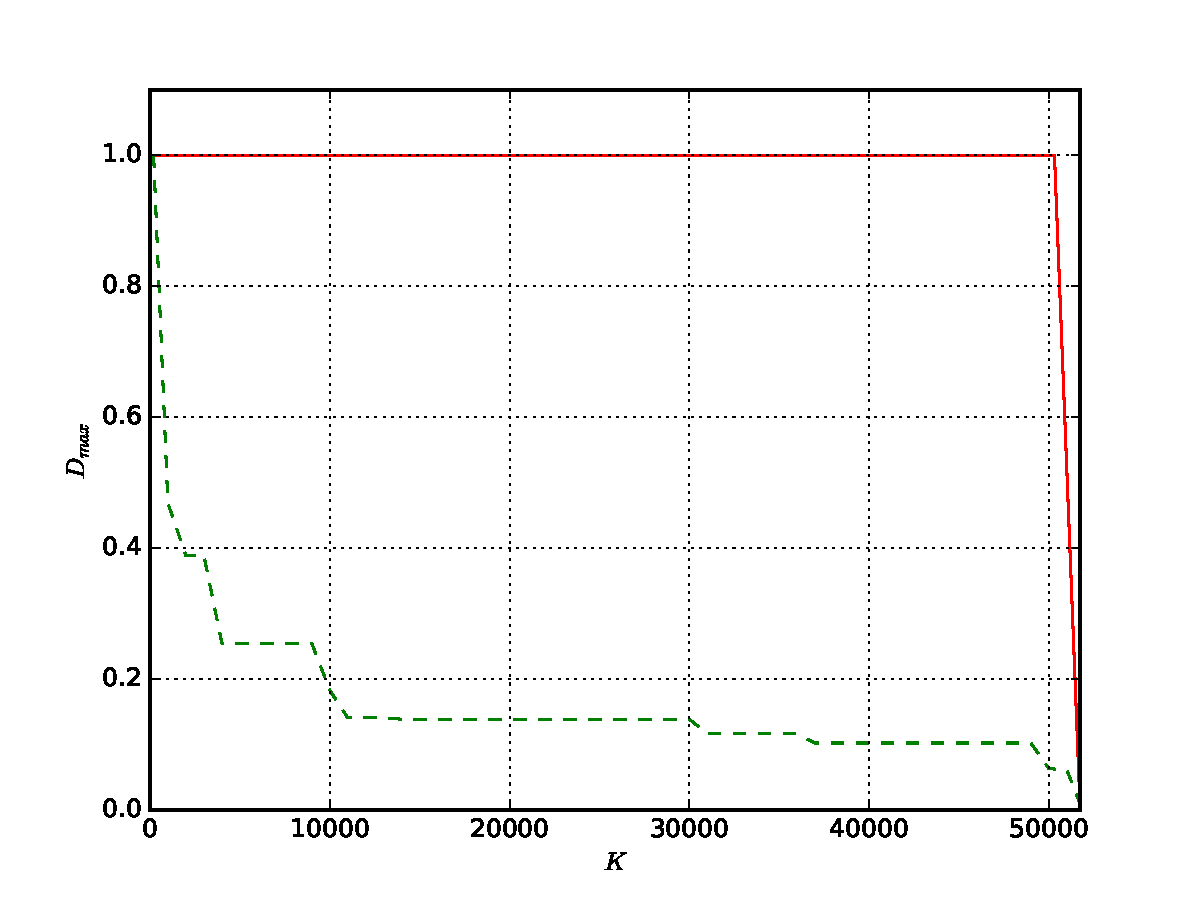
\includegraphics[width=.5\textwidth]{mixed_2d_max.pdf}}}
    \subfloat[\(D_{avg}\)]{
    \label{fig:avg_dev} {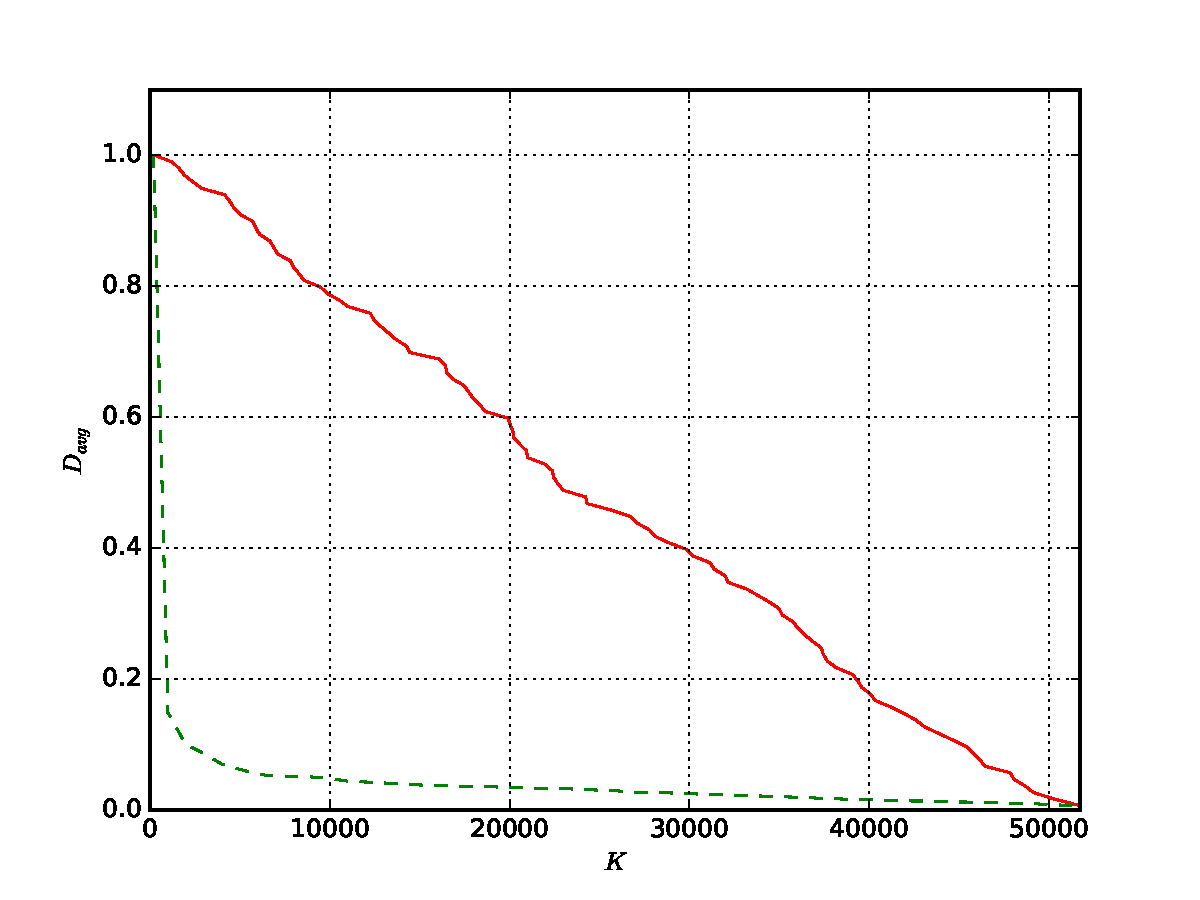
\includegraphics[width=.5\textwidth]{mixed_2d_avg.pdf}}}
    \caption{Динамика величин \(D_{avg}\) и \(D_{max}\) в процессе решения множества двухмерных задач,
    порождённых двумя разными генераторами GKLS и \(F_{GR}\)}
    \label{fig:devs_mixed}
\end{figure}

\subsubsection{Пример решения многокритериальной задачи}

Для демонстрации эффективности подхода к балансировке нагрузки рассмотрим пример,
в котором множество задач вида (\ref{eq:many_problems}) порождено в результате скаляризации
многокритериальной задачи оптимизации с ограничениями.

Рассмотрим тестовую задачу, предложенную в \cite{BinhKorn1999}:
\begin{equation}
  \label{eq:mco_probem}
  \begin{array}{l}
      Minimize \left \{
      \begin{array}{l}
        f_1(y) = 4 y_1^2 + 4 y_2^2 \\
        f_2(y) = (y_1-5)^2 + (y_2-5)^2 \\
      \end{array}
      \right .
      y_1\in [-1;2],y_2\in [-2;1]
      \\s.t.
      \\
      \left \{
      \begin{array}{l}
        g_1(y) = (y_1 - 5)^2 + y_2^2 - 25 \leqslant 0 \\
        g_2(y) = -(y_1 - 8)^2 - (y_2 + 3)^2 + 7.7 \leqslant 0\\
      \end{array}
      \right .
  \end{array}
\end{equation}

Будем использовать свертку Гермейера для скаляризации задачи (\ref{eq:mco_probem}).
После свертки скалярная целевая функция имеет вид:
\begin{equation}
  \varphi(y,\lambda_1,\lambda_2)=\max\{\lambda_1 f_1(y), \lambda_2 f_2(y)\},
\end{equation}
где \(\lambda_1,\lambda_2\in[0,1],\: \lambda_1+\lambda_2=1\). Перебирая все возможные
коэффициенты свертки, можно найти все множество парето-оптимальных решений в
задаче (\ref{eq:mco_probem}). Для численного построения множества Парето выберем
100 наборов коэффициентов \((\lambda_1,\lambda_2)\) таких, что
\(\lambda_1^i=i h,\: \lambda_2^i=1-\lambda_1^i,\: h=10^{-2},i=\overline{1, 100}\).

В качестве ограничения на вычислительные ресурсы был выбран лимит в 2500 испытаний.
Множество вспомогательных скалярных задач решалось двумя способами:
\begin{itemize}
  \item каждая задача решается отдельно с помощью IAGS с установленным лимитом в
  25 испытаний. Таким образом, вычислительные ресурсы равномерно распределены между задачами;
  \item все задачи решаются одновременно с помощью обобщенного IAGS с установленным лимитом в
  2500 испытаний.
\end{itemize}
В обоих случаях параметр \(r=4\).

\begin{figure}[ht]
    \centering
    \subfloat[IAGS, раздельное решение задач]{
    \label{fig:mco_pareto_1} {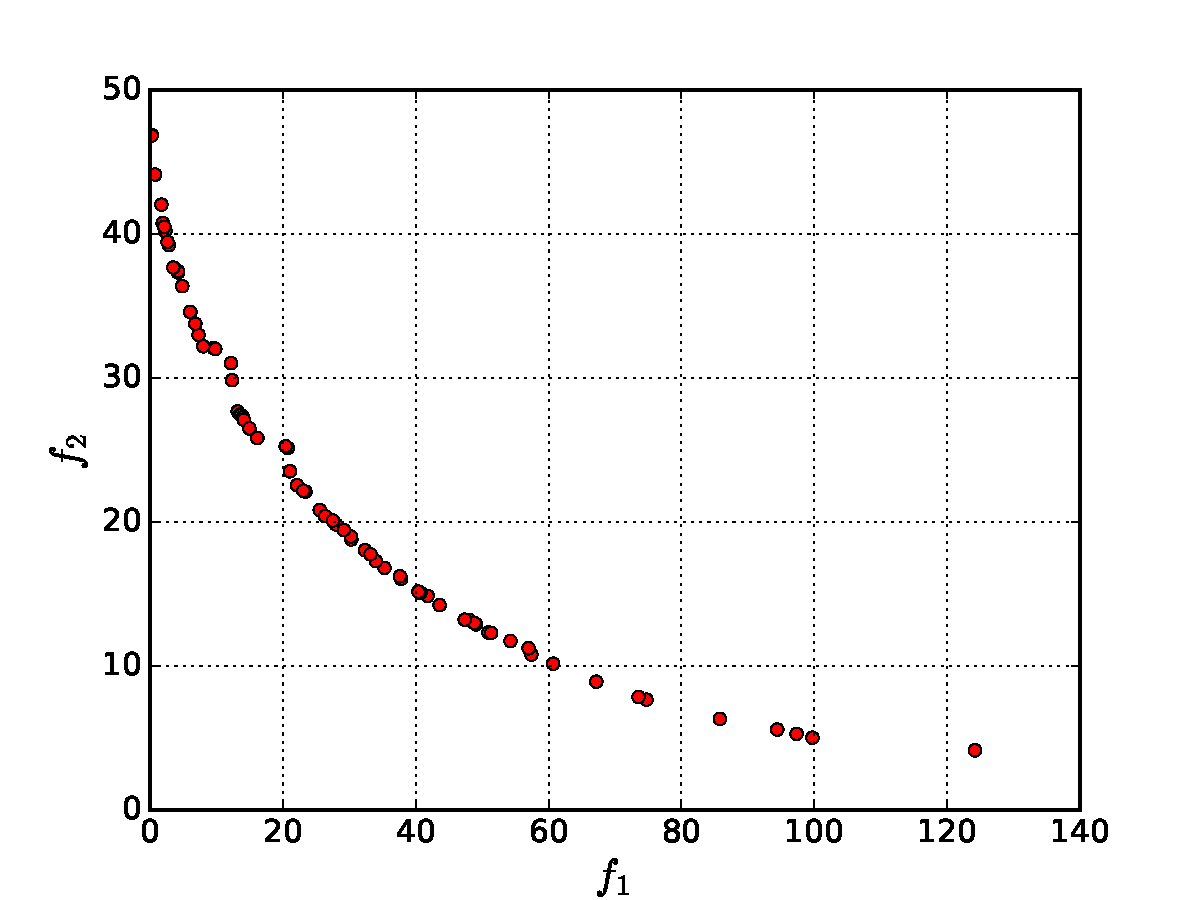
\includegraphics[width=.5\textwidth]{single_mco.pdf}}}
    \subfloat[IAGS для множества задач]{
    \label{fig:mco_pareto_2} {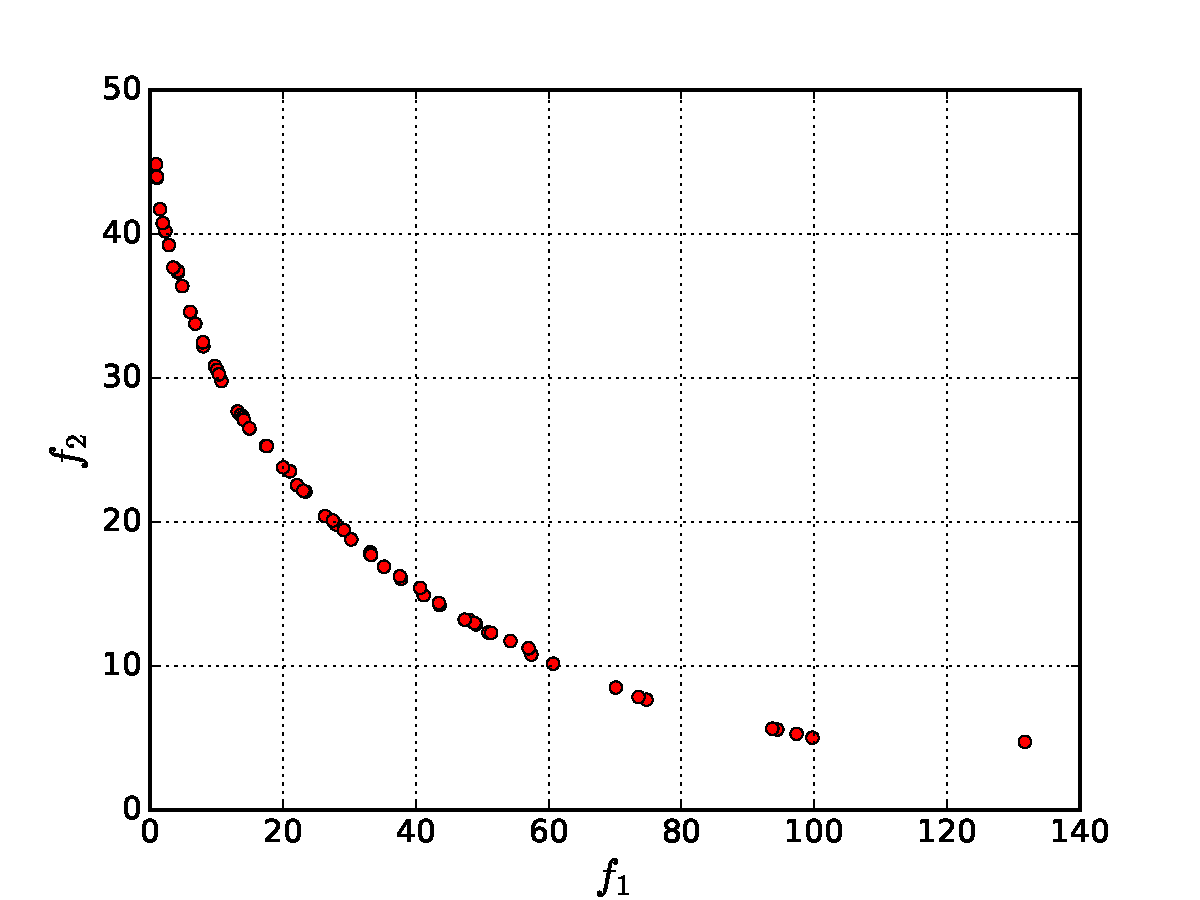
\includegraphics[width=.5\textwidth]{multi_mco.pdf}}}
    \caption{Численные оценки множества Парето в задаче (\ref{eq:mco_probem}), полученные после 2500 испытаний}
    \label{fig:mco_pareto}
\end{figure}

На рис. \ref{fig:mco_pareto} представлены графики решений, полученных каждым из методов.
Все графики качественно совпадают с указанным в \cite{BinhKorn1999} (авторы не предоставили другой
информации и решениях для сравнения). Видно, что на рис. \ref{fig:mco_pareto_1}
кривая Парето имеет вогнутости, что не соответствует решению, указанному в \cite{BinhKorn1999} и
означает нехватку ресурсов для решения некоторых из вспомогательных задач.
Для оценки качества решения также был вычислен показатель \(Spacing(SP)\) \cite{RiquelmeLucken2015},
характеризующий плотность точек аппроксимации множества Парето.
\begin{displaymath}
  SP(S)=\sqrt{\frac{1}{|S|-1} \sum_{i=1}^{|S|} (\overline{d}-d_i)^2},
  \; \overline{d}=mean\{d_i\},
  \\d_i=\min_{s_i,s_j\in S:s_i\ne s_j}||F(s_i)-F(s_j)||_1,\; F=(f_1,f_2).
\end{displaymath}
В случае отдельного решения задач \(SP_{single}=0.984\), а при решении задач методом с балансировкой нагрузки
\(SP_{multi}=0.749\), что говорит о более качественном приближении решения.

\subsection{Итоги}

В данном разделе была реализована поддержка нелинейных ограничений в алгоритме, решающeм
множество задач глобальной оптимизации в совокупности и распределяющего свои ресурсы так, чтобы
обеспечивать равномерную сходимость во всех задачах. Доказано теорема о достаточных условиях сходимости
полученного метода. Свойство равномерной сходимости проверено с помощью численного эксперимента.
Также в ходе численных экспериментов была оценена эффективность выполненной параллельной реализации метода и
показана эффективность совместного решения множества задач на примере получения Парето фронта в многокритериальной задаче с
нелинейными ограничениями.
